\documentclass[
	% -- opções da classe memoir --
	12pt,				  % tamanho da fonte
	openright,	  % capítulos começam em pág ímpar (insere página vazia caso preciso)
	oneside,			% para impressão em recto e verso. Oposto a oneside
	a4paper,			% tamanho do papel. 
	% -- opções da classe abntex2 --
	%chapter=TITLE,		% títulos de capítulos convertidos em letras maiúsculas
	%section=TITLE,		% títulos de seções convertidos em letras maiúsculas
	%subsection=TITLE,	% títulos de subseções convertidos em letras maiúsculas
	%subsubsection=TITLE,% títulos de subsubseções convertidos em letras maiúsculas
	% -- opções do pacote babel --
	english,			% idioma adicional para hifenização
	french,				% idioma adicional para hifenização
	spanish,			% idioma adicional para hifenização
	brazil				% o último idioma é o principal do documento
	]{abntex2}

% ---
% Pacotes básicos 
% ---
\usepackage{lmodern}			% Usa a fonte Latin Modern			
\usepackage[T1]{fontenc}		% Selecao de codigos de fonte.
\usepackage[utf8]{inputenc}	% Codificacao do documento (conversão automática dos acentos)
\usepackage{lastpage}		% Usado pela Ficha catalográfica
\usepackage{indentfirst}		% Indenta o primeiro parágrafo de cada seção.
\usepackage{color}			% Controle das cores
\usepackage{graphicx}		% Inclusão de gráficos
\usepackage{microtype} 		% para melhorias de justificação
\usepackage{lipsum}			% Gera texto dummy
\usepackage{lscape}			% Página na horizontal
\usepackage{xspace}
\usepackage{tikz}
\usetikzlibrary{positioning}
\usepackage{multirow}
\usepackage{array}
\usepackage{graphicx}
\usepackage{pdfpages}
% ---

% ---
% Pacotes de citações
% ---
\usepackage[brazilian,hyperpageref]{backref}	 % Paginas com as citações na bibl
\usepackage[alf]{abntex2cite}	% Citações padrão ABNT

% --- 
% CONFIGURAÇÕES DE PACOTES
% --- 

% ---
% Configurações do pacote backref
% Usado sem a opção hyperpageref de backref
\renewcommand{\backrefpagesname}{Citado na(s) página(s):~}
% Texto padrão antes do número das páginas
\renewcommand{\backref}{}
% Define os textos da citação
\renewcommand*{\backrefalt}[4]{
	\ifcase #1 %
		Nenhuma citação no texto.%
	\or
		Citado na página #2.%
	\else
		Citado #1 vezes nas páginas #2.%
	\fi}%
% ---

% ---
% Informações de dados para CAPA e FOLHA DE ROSTO
% ---
\titulo{Título da tese ou dissertação}
\autor{Nome do autor}
\local{Rio de Janeiro}
\data{2021}
\orientador{Nome do orientador}
\coorientador{Nome do co-orientador}
\instituicao{%
  Fundação Oswaldo Cruz
  \par
  Instituto de Comunicação e Informação Científica e Tecnológica em Saúde
  \par
  Programa de Pós-Graduação em Informação e Comunicação em Saúde}
\tipotrabalho{Tese (doutorado)}
% O preambulo deve conter o tipo do trabalho, o objetivo, 
% o nome da instituição e a área de concentração 
\preambulo{Tese apresentada ao Programa de Pós-Graduação em Informação e Comunicação em Saúde do Instituto de Comunicação e Informação em Saúde (Icict) para obtenção do grau de Doutor/Mestre em Ciências.}
% ---

% ---
% Comandos para texto formatado
% ---
\newcommand{\bigdata}{\emph{big data}\xspace}
\newcommand{\cdados}{\emph{ciência de dados}\xspace}
\newcommand{\cdadossaude}{\emph{ciência de dados em saúde}\xspace}
\newcommand{\estatistica}{\emph{estatística}\xspace}
\newcommand{\SaudePublica}{\emph{Saúde Pública}\xspace}
\newcommand{\bul}{$\bullet$\xspace}
% ---

% ---
% Configurações de epígrafe
% ---
\setlength\epigraphwidth{.8\textwidth}
\setlength\epigraphrule{0pt}
% ---

% ---
% Capa
% ---
\renewcommand{\imprimircapa}{%
  \begin{capa}%
    \center
	\begin{minipage}{.5\textwidth}
	  \flushleft
	  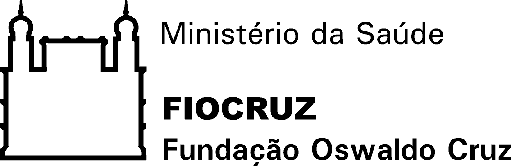
\includegraphics[scale=.3]{img/logo_friocruz.png}
	\end{minipage}%
	\begin{minipage}{.5\textwidth}
	  \flushright
	  
\includegraphics[scale=.25]{img/logo_icict.png} 
	\end{minipage}\\
    \vspace{4cm}
    {\ABNTEXchapterfont\large\imprimirautor}
    \vspace{3cm}
    \begin{center}
    \ABNTEXchapterfont\bfseries\LARGE\imprimirtitulo
    \end{center}    
    \vspace{5cm}
    \vfill
    \large\imprimirlocal\\
    \large\imprimirdata
    \vspace*{1cm}
  \end{capa}
}
% ---

% ---
% Folha de rosto
% ---
\renewcommand{\folhaderostocontent}{%
  \begin{capa}%
    \center
    {\ABNTEXchapterfont\large\imprimirautor}
    \vspace*{\fill}
    \begin{center}
    \ABNTEXchapterfont\bfseries\LARGE\imprimirtitulo
    \end{center} 
    \vspace*{\fill}   
    \hspace{.45\textwidth}
    \begin{minipage}{.5\textwidth}
     \SingleSpacing
      \imprimirpreambulo\\

      Orientador: \imprimirorientador\\
      Co-orientador: \imprimircoorientador\\
    \end{minipage}%
    \vspace*{\fill}
    \large\imprimirlocal\\
    \large\imprimirdata
  \end{capa}
}
% ---




% ---
% Configurações para quadro
% ---
\newcommand{\quadroname}{Quadro}
\newcommand{\listofquadrosname}{Lista de quadros}
\newfloat[chapter]{quadro}{loq}{\quadroname}
\newlistof{listofquadros}{loq}{\listofquadrosname}
\newlistentry{quadro}{loq}{0}
% configurações para atender às regras da ABNT
\setfloatadjustment{quadro}{\centering}
\counterwithout{quadro}{chapter}
\renewcommand{\cftquadroname}{\quadroname\space} 
\renewcommand*{\cftquadroaftersnum}{\hfill--\hfill}
% Configuração de posicionamento padrão:
\setfloatlocations{quadro}{hbtp}
% ---


% ---
% Configurações de aparência do PDF final

% alterando o aspecto da cor azul
\definecolor{blue}{RGB}{41,5,195}

% informações do PDF
\makeatletter
\hypersetup{
     	%pagebackref=true,
		pdftitle={\@title}, 
		pdfauthor={\@author},
    	pdfsubject={\imprimirpreambulo},
	    pdfcreator={LaTeX with abnTeX2},
		pdfkeywords={abnt}{latex}{abntex}{abntex2}{trabalho acadêmico}, 
		colorlinks=true,       		% false: boxed links; true: colored links
    	linkcolor=blue,          	% color of internal links
    	citecolor=blue,        		% color of links to bibliography
    	filecolor=magenta,      		% color of file links
		urlcolor=blue,
		bookmarksdepth=4
}
\makeatother
% --- 

% --- 
% Espaçamentos entre linhas e parágrafos 
% --- 

% O tamanho do parágrafo é dado por:
\setlength{\parindent}{1.3cm}

% Controle do espaçamento entre um parágrafo e outro:
\setlength{\parskip}{0.2cm}  % tente também \onelineskip

% ---
% compila o índice
% ---
\makeindex
% ---

% ----
% Início do documento
% ----
\begin{document}

% Seleciona o idioma do documento (conforme pacotes do babel)
%\selectlanguage{english}
\selectlanguage{brazil}

% Retira espaço extra obsoleto entre as frases.
\frenchspacing 

% ----------------------------------------------------------
% ELEMENTOS PRÉ-TEXTUAIS
% ----------------------------------------------------------
% \pretextual

% ---
% Capa
% ---
\imprimircapa
% ---

% ---
% Folha de rosto
% (o * indica que haverá a ficha bibliográfica)
% ---
\imprimirfolhaderosto*
% ---

% Ficha catalográfica da Fiocruz
% https://www.boletimdigital.icict.fiocruz.br/ficha_Bib_Mang/

\includepdf[]{ficha.pdf}

% ---
% Inserir folha de aprovação
% ---

% Isto é um exemplo de Folha de aprovação, elemento obrigatório da NBR
% 14724/2011 (seção 4.2.1.3). Você pode utilizar este modelo até a aprovação
% do trabalho. Após isso, substitua todo o conteúdo deste arquivo por uma
% imagem da página assinada pela banca com o comando abaixo:
%
% \begin{folhadeaprovacao}
% \includepdf{folhadeaprovacao_final.pdf}
% \end{folhadeaprovacao}
%

\begin{folhadeaprovacao}

  \begin{center}
    \imprimirinstituicao\\
	\vspace*{\fill}\vspace*{\fill}
    {\ABNTEXchapterfont\large\imprimirautor}
    \vspace*{\fill}\vspace*{\fill}
    \begin{center}
      \ABNTEXchapterfont\bfseries\Large\imprimirtitulo
    \end{center}
    \vspace*{\fill}
   \end{center}
        
   Aprovado em 23 de fevereiro de 2021.

   \assinatura{\textbf{\imprimirorientador} \\ Orientador} 
   \assinatura{\textbf{\imprimircoorientador} \\ Co-Orientador} 
   \assinatura{\textbf{Componente da banca 1}}
   \assinatura{\textbf{Componente da banca 2}}
   \assinatura{\textbf{Componente da banca 3}}
   \assinatura{\textbf{Componente da banca 4}}
      
   \begin{center}
    \vspace*{0.5cm}
    {\large\imprimirlocal}
    \par
    {\large\imprimirdata}
    \vspace*{1cm}
  \end{center}
  
\end{folhadeaprovacao}
% ---

% ---
% Dedicatória
% ---
\begin{dedicatoria}
   \vspace*{\fill}
   \centering
   \noindent
   \textit{Dedicatória...} \vspace*{\fill}
\end{dedicatoria}
% ---

% ---
% Agradecimentos
% ---
\begin{agradecimentos}
Agradecimentos...

\end{agradecimentos}

% ---
% Epígrafe
% ---
\begin{epigrafe}
    \vspace*{\fill}
	\begin{flushright}
		\textit{Epígrafe...\\
		(Autor da epígrafe)}
	\end{flushright}
\end{epigrafe}
% ---

% ---
% Resumo em língua vernácula
% ---
% resumo em português
\setlength{\absparsep}{18pt} % ajusta o espaçamento dos parágrafos do resumo
\begin{resumo}
 Resumo em português...

 \textbf{Palavras-chave}: Ciência de Dados. Métodos epidemiológicos. Saúde Pública.
\end{resumo}

% resumo em inglês
\begin{resumo}[Abstract]
 \begin{otherlanguage*}{english}
   Resumo em inglês...

   \vspace{\onelineskip}
 
   \noindent 
   \textbf{Keywords}: Data Science. Epidemiological methods. Public health. 
 \end{otherlanguage*}
\end{resumo}

% ---
% inserir lista de ilustrações
% ---
\pdfbookmark[0]{\listfigurename}{lof}
\listoffigures*
\cleardoublepage
% ---

% ---
% inserir lista de tabelas
% ---
\pdfbookmark[0]{\listtablename}{lot}
\listoftables*
\cleardoublepage
% ---

% ---
% inserir lista de quadros
% ---
\pdfbookmark[0]{\listofquadrosname}{loq}
\listofquadros*
\cleardoublepage
% ---

% ---
% inserir lista de abreviaturas e siglas
% ---
\begin{siglas}
  \item[ANA] Agência Nacional das Águas
  \item[ANM] Agência Nacional de Mineração
  \item[API] \emph{Application Programming Interface}
\end{siglas}
% ---

% ---
% inserir lista de símbolos
% ---
%\begin{simbolos}
%  \item[$ \Gamma $] Letra grega Gama
%  \item[$ \Lambda $] Lambda
%  \item[$ \zeta $] Letra grega minúscula zeta
%  \item[$ \in $] Pertence
%\end{simbolos}
% ---

% ---
% inserir o sumario
% ---
\settocdepth{section}
\pdfbookmark[0]{\contentsname}{toc}
\tableofcontents*
\cleardoublepage
% ---


% ----------------------------------------------------------
% ELEMENTOS TEXTUAIS
% ----------------------------------------------------------
\textual

% ---
% Introdução
% ---% 
%\chapter*[Introdução]{Introdução}
%\addcontentsline{toc}{chapter}{Introdução}
\chapter{Introdução}
% ---



% ---
% Objetivos
% ---
\clearpage
\section{Objetivos}
\label{sec:objetivos}
% ---

\subsection*{Objetivo geral}


% ---
% Estrutura da tese
% ---
%\clearpage
\section{Estrutura da tese}
\label{sec:estrutura_da_tese}
% ---



% ---
% Referencial teórico
% ---
\chapter{Referencial teórico}
\label{ch:referencial_teorico}
% ---

\epigraph{\itshape Va, pensiero, sull'ali dorate; 
Va, ti posa sui clivi, sui colli, 
Ove olezzano tepide e molli 
L'aure dolci del suolo natal!}{---Verdi, \emph{Nabucco}.}


\section{Seção...}



\subsection*{Subseção não numerada...}

\begin{citacao}[english]
Citação direta em inglês...
\end{citacao}

Exemplo de quadro:

\newpage
\begin{landscape}
\begin{quadro}[h!]
\caption{\label{quadro:eras_epidemiologia} Eras da evolução da epidemiologia}
\small
\begin{tabular}{|p{5cm}|p{4.2cm}|p{4.2cm}|p{4.2cm}|p{4.2cm}|}
\hline 
Era & Paradigma & Procedimento analítico & Procedimento preventivo & Dados \\ 
\hline 
Estatística Sanitária (primeira metade do século XIX) & Miasma: envenenamento por emanações do solo, ar e água. & Demonstrar agrupamentos de morbidade e mortalidade. & Saneamento, abastecimento canalizado, medidas sanitárias. & Dados secundários, registros de mortalidade das paróquias. \\ 
\hline 
Doenças Infecciosas (final do século XIX até meados do século XX) & Teoria dos germes: agentes únicos relacionados a doenças específicas. & Isolamento laboratorial e criação de culturas, experimentos com transmissão de doenças e reprodução de lesões. & Interromper a transmissão, vacinas, isolamento dos doentes em quarentenas e hospitais específicos. & Dados primários e secundários, inquéritos e levantamentos por doenças específicas. \\ 
\hline 
Epidemiologia de doenças crônicas (meados do século XX) & Caixa preta: exposição relacionada ao desfecho, sem necessidade de fatores intervenientes ou patogenia. & Razão de risco de fatores em relação a um desfecho no nível individual. & Controlar os fatores de risco modificando o estilo de vida (dieta, exercícios, etc.), agente (armas, trânsito, etc.) e meio ambiente (poluição, fumo passivo, etc). & Ênfase nos dados secundários, cruzamentos de fontes de dados sociais. \\ 
\hline 
Eco-Epidemiologia (emergente) & Caixas chinesas: relações entre e através de estruturas organizadas hierarquicamente. & Análise de determinantes e desfechos em diferentes níveis de organização: dentro e entre contextos (sistemas de informação) e em profundidade (técnicas da biomedicina). & Aplicar tecnologias biomédicas e da informação, do nível contextual ao molecular. & Dados primários e secundários, dados individuais e agregados. \\ 
\hline 
Ciência de dados & \bigdata: métodos de predição não explicativos e não autoexplicativos. & ETL, mineração de dados, visualização de dados complexos e predição de desfechos. & Medicina de precisão, procedimentos individualizados, predição de cenários. & Grandes bases de dados estruturadas e não estruturadas, prontuários eletrônicos, internet das coisas. \\ 
\hline 
\end{tabular}{ 
\footnotesize
\\Fonte: adaptado de \citeonline{Susser1996, Susser1996a, Susser2009, Chiavegatto2015}.
}
\end{quadro}
\end{landscape}
\newpage





% ---
% Metodologia
% ---
\chapter{Metodologia}
\label{ch:metodologia}
% ---

Exemplo de figura...

\begin{figure}[htb]
  \caption{\label{fig:processo_kdd}O processo KDD}
  \begin{center}
    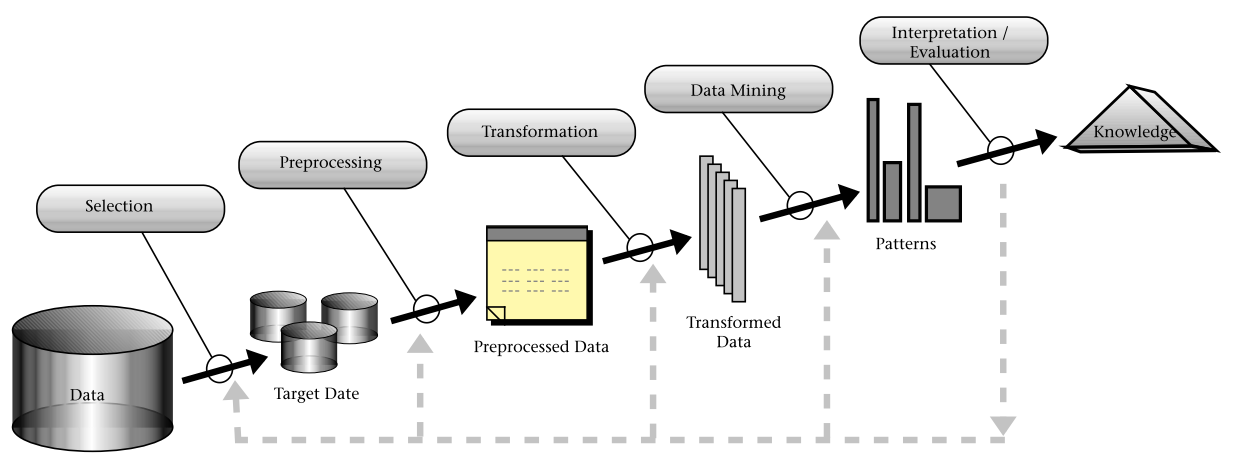
\includegraphics[width=.8\textwidth]{img/processo_kdd.png}
  \end{center}
  \legend{Fonte: \citeonline{Fayyad1996}}
\end{figure}


Exemplo de tabela

\begin{table}[htb]
\caption{\label{tabela:sistemas_volume} Volume de alguns sistemas de informação de saúde nacionais}
\small
\centering
\begin{tabular}{ccc}
\hline 
Sistema & Período & Registros \\ 
\hline
SIA & 1994 a 2017 & 63.987.334.421 \\
SIH & 1984 a 2018 & 403.452.248 \\
SINASC & 1994 a 2017 & 71.270.156 \\
CNES & 2005 a 2018 & 38.223.272\\
SIM & 1979 a 2017 &  37.372.780 \\
\hline 
\end{tabular} 
{
\footnotesize
\\Fonte: compilado pelo autor com dados do DataSUS.
}
\end{table}


% ---
% Resultados
% ---
\chapter{Resultados}
\label{ch:resultados}
% ---



% ---
% Conclusão
% ---% 
\chapter{Conclusão}
\label{ch:conclusao}
% ---% 

\epigraph{\itshape Religion is a culture of faith; science is a culture of doubt.}{---Richard Feynman}













% ----------------------------------------------------------
% ELEMENTOS PÓS-TEXTUAIS
% ----------------------------------------------------------
\postextual
% ----------------------------------------------------------

% ----------------------------------------------------------
% Referências bibliográficas
% ----------------------------------------------------------
\bibliography{library.bib}

% ----------------------------------------------------------
% Glossário
% ----------------------------------------------------------
%
% Consulte o manual da classe abntex2 para orientações sobre o glossário.
%
%\glossary

% ----------------------------------------------------------
% Apêndices
% ----------------------------------------------------------


%% ---
%
%
%% ----------------------------------------------------------
%% Anexos
%% ----------------------------------------------------------
%
%% ---
%% Inicia os anexos
%% ---
%\begin{anexosenv}
%
%% Imprime uma página indicando o início dos anexos
%\partanexos
%
%% ---
%\chapter{Morbi ultrices rutrum lorem.}
%% ---
%\lipsum[30]
%
%% ---
%\chapter{Cras non urna sed feugiat cum sociis natoque penatibus et magnis dis
%parturient montes nascetur ridiculus mus}
%% ---
%
%\lipsum[31]
%
%% ---
%\chapter{Fusce facilisis lacinia dui}
%% ---
%
%\lipsum[32]
%
%\end{anexosenv}

%---------------------------------------------------------------------
% INDICE REMISSIVO
%---------------------------------------------------------------------
%\phantompart
%\printindex
%---------------------------------------------------------------------



%---------------------------------------------------------------------
% COLOFÃO
%---------------------------------------------------------------------

\pagebreak\thispagestyle{empty}
~\vfill{}
\noindent
\begin{center}
Este documento foi digitado e diagramado utilizando as tecnologias \TeX{}, \LaTeX{}, \TeX{}Live e \TeX{}Maker; com estilos providos pela classe \textsc{abn}\TeX2. \\
\bigskip{}
\emph{Gerado em \today.}
\end{center}

\end{document}
